\documentclass[11pt,a4paper]{article}
\usepackage[T1]{fontenc}
\usepackage[utf8]{inputenc}
\usepackage[brazil]{babel}
\usepackage{lmodern}
\usepackage{microtype}
\usepackage[a4paper,margin=2.5cm]{geometry}
\usepackage{graphicx}
\usepackage{booktabs}
\usepackage{tabularx}
\usepackage{array}
\usepackage{float}
\usepackage{caption}
\usepackage{rotating}
\usepackage{tikz}
\usetikzlibrary{arrows.meta,positioning}
\usepackage[hidelinks]{hyperref}
\usepackage{parskip}

\captionsetup{font=small,labelfont=sc}
\newcolumntype{L}{>{\raggedright\arraybackslash}X}
\renewcommand{\arraystretch}{1.25}

% Foto do protótipo: usa o arquivo se ele existir, senão mostra um quadro reservado.
\newcommand{\foto}[3]{%
  \begin{figure}[H]\centering
  \IfFileExists{#1}{\includegraphics[width=0.8\linewidth]{#1}}%
  {\fbox{\parbox[c][5.5cm][c]{0.78\linewidth}{\centering\small Espaço reservado para a fotografia\\[2pt]\texttt{\detokenize{#1}}}}}
  \caption{#2}\label{#3}\end{figure}}

\title{\vspace{-1cm}\normalsize Universidade de São Paulo\\Escola Politécnica\\Departamento de Engenharia de Computação e Sistemas Digitais\\[4pt]PCS3848 Sistemas Embarcados\\[2.2cm]
\LARGE Projeto Talos\\[4pt]\large Cofre eletrônico com ESP32\\[6pt]\normalsize Relatório técnico de progresso do projeto dirigido\\[2cm]}
\author{André Moreno (13682785)\\Felipe Soria (13864287)\\Giovani Sebastianutti (13680171)\\Matheus Guidoni (12683120)}
\date{São Paulo, outubro de 2026}

\begin{document}
\begin{titlepage}
\maketitle
\thispagestyle{empty}
\end{titlepage}

\begin{abstract}
Este relatório descreve o progresso do Projeto Talos desde o início da disciplina. O projeto constrói um cofre eletrônico que destrava uma fechadura solenoide quando o usuário digita uma senha de seis dígitos em um teclado matricial. Um microcontrolador ESP32 executa uma máquina de estados que aplica um desafio anti-marcas antes da senha, bloqueia o teclado após tentativas inválidas com tempo crescente, guarda a senha como hash SHA-256 em memória não volátil com cópia dupla e verificação por CRC32 e mantém o sistema em deep sleep quando ninguém o usa. O texto apresenta os requisitos e o estado de cada um, a arquitetura do produto, do hardware e do software, o projeto detalhado, os protocolos de comunicação, as ferramentas, a interface com o usuário, o protótipo atual, os problemas que o grupo enfrentou e o cronograma.
\end{abstract}

\tableofcontents
\newpage

\section{Introdução}

O Projeto Talos nasceu de uma especificação que o grupo escreveu na forma de monografia no início da disciplina. A monografia define um cofre eletrônico para uso residencial e em pequenos comércios, com baixo custo, operação simples e alimentação por bateria. O usuário acorda o cofre com qualquer tecla, digita dois dígitos aleatórios que o cofre sorteia, digita a senha e confirma. Com a senha correta, a fechadura destrava por alguns segundos e depois trava de novo.

Desde a especificação, o grupo escolheu e comprou os componentes principais, escreveu e testou o firmware em uma placa ESP32 DevKit V1, produziu um guia de montagem e um guia de testes e enfrentou problemas práticos que mudaram partes do projeto original. A fechadura comprada, por exemplo, exige uma tensão bem maior que a bateria de lítio da monografia, o que levou o grupo a adotar uma bateria de 9 V. Este relatório registra essas decisões, o estado atual de cada parte e o que ainda falta.

\section{Especificação de requisitos}

A monografia lista dezessete requisitos funcionais e sete requisitos não funcionais. As tabelas \ref{tab:rf} e \ref{tab:rnf} reproduzem cada requisito de forma resumida e indicam o estado atual da implementação. O grupo considera um requisito implementado quando o firmware já o cumpre e algum teste na placa já o exercitou. Um requisito parcial cumpre a ideia central com alguma diferença em relação ao texto original, e um requisito pendente ainda depende de hardware ou de montagem.

\begin{table}[H]\centering\small
\caption{Requisitos funcionais e estado atual.}\label{tab:rf}
\begin{tabularx}{\linewidth}{@{}l L l@{}}
\toprule
Código & Requisito & Estado \\
\midrule
RF-01 & Cada toque gera exatamente um evento (debounce de 50 ms) & Implementado \\
RF-02 & Descartar a entrada parcial após 15 s sem interação & Implementado \\
RF-03 & Bloquear o teclado após 5 senhas erradas & Implementado \\
RF-04 & Dobrar o tempo de bloqueio em bloqueios consecutivos, até 30 min & Implementado \\
RF-05 & Destravar a fechadura com a senha correta & Implementado \\
RF-06 & Trocar a senha por um fluxo controlado & Parcial \\
RF-07 & Exigir dois dígitos aleatórios antes da senha (desafio anti-marcas) & Implementado \\
RF-08 & Sinalizar cada evento com um padrão sonoro distinto & Implementado \\
RF-10 & Permitir a troca da bateria sem ferramentas & Pendente \\
RF-11 & Avisar quando a bateria estiver fraca & Parcial \\
RF-12 & Entrar em deep sleep sem interação & Implementado \\
RF-13 & Acordar com qualquer tecla & Implementado \\
RF-14 & Modo stealth, sem som & Implementado \\
RF-15 & Aceitar a confirmação só com 6 dígitos & Implementado \\
RF-16 & Manter senha e configurações sem bateria & Implementado \\
RF-17 & Trancar ao detectar o fechamento da porta & Pendente \\
RF-18 & Indicar o sucesso da autenticação & Implementado \\
\bottomrule
\end{tabularx}
\end{table}

O RF-06 está parcial porque o grupo trocou a janela de 60 s após a autenticação por uma janela mais simples. A troca de senha começa quando o usuário aperta a tecla A durante os 5 s em que a fechadura está aberta. O modo por jumper interno não entrou no firmware. O RF-11 está parcial porque o firmware já mede a bateria e avisa abaixo de 7 V, mas o divisor resistivo ainda não faz parte da montagem. O RF-10 depende da montagem no case e o RF-17 depende de um sensor de porta que o grupo ainda não comprou. O firmware já trata o sensor e só precisa que alguém ative a constante correspondente.

\begin{table}[H]\centering\small
\caption{Requisitos não funcionais e estado atual.}\label{tab:rnf}
\begin{tabularx}{\linewidth}{@{}l L l@{}}
\toprule
Código & Requisito & Estado \\
\midrule
RNF-01 & Voltar a um estado seguro após qualquer reset & Implementado \\
RNF-02 & Não expor informação útil a um atacante & Implementado \\
RNF-03 & Proteger a memória não volátil contra corrupção & Implementado \\
RNF-04 & Dar retorno claro para todas as ações & Implementado \\
RNF-05 & Durar pelo menos 2 anos com uma bateria & Parcial \\
RNF-06 & Usar o mínimo de componentes externos & Implementado \\
RNF-07 & Carcaça resistente e eletrônica inacessível & Pendente \\
\bottomrule
\end{tabularx}
\end{table}

O RNF-02 abrange quatro cuidados que o firmware já aplica. Ele guarda apenas o hash SHA-256 da senha, compara os hashes em tempo constante, nunca escreve a senha no log serial e grava o contador de tentativas antes de qualquer sinal de erro, para que desligar a energia ao ouvir o bipe de erro não apague a tentativa. O RNF-05 continua parcial porque a placa de desenvolvimento consome alguns miliampères mesmo em deep sleep, por causa do LED de energia, do regulador e do conversor USB. Com uma bateria de 9 V comum, a autonomia fica em poucos dias. A meta de dois anos exige um ESP32 sem a placa de desenvolvimento, o que o grupo deixa como trabalho futuro.

\section{Arquitetura}

\subsection{Produto}

O produto final é uma caixa de MDF com o teclado na tampa e a fechadura solenoide alinhada ao batente. A placa ESP32, o MOSFET que aciona a fechadura e o buzzer ficam dentro da caixa. A bateria fica em um compartimento acessível por fora, como pede o RF-10. Um módulo de display de seis dígitos, ainda a caminho, vai mostrar o desafio e a senha durante a digitação.

\subsection{Hardware}

A figura \ref{fig:blocos} mostra os blocos de hardware. O ESP32 lê o teclado por oito fios, aciona a fechadura por meio de um MOSFET, aciona o buzzer diretamente por um pino e vai conversar com o display por dois fios. Uma única bateria de 9 V alimenta a placa pelo pino VIN e alimenta a fechadura diretamente. Um divisor resistivo opcional leva a tensão da bateria até uma entrada analógica.

\begin{figure}[H]\centering
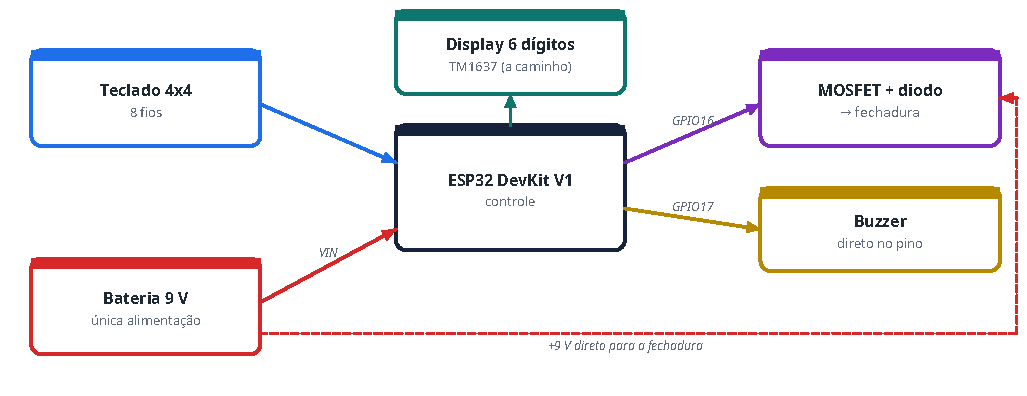
\includegraphics[width=0.85\linewidth]{figuras/blocos.pdf}
\caption{Blocos de hardware do sistema.}\label{fig:blocos}
\end{figure}

\subsection{Software}

O software segue a divisão que a monografia propõe entre fluxo de dados e unidade de controle. O fluxo de dados reúne as rotinas que tocam o hardware: varredura do teclado com debounce, geração do desafio, comparação de hashes, contador de tentativas com cálculo do bloqueio, temporizadores, saída de som e luz, acionamento da fechadura, leitura da bateria e driver do display. A unidade de controle é uma máquina de estados finitos que recebe os eventos dessas rotinas e decide a próxima ação. A figura \ref{fig:fsm} mostra os estados e as transições da versão atual.

\begin{figure}[H]\centering
\begin{tikzpicture}[>=Stealth, node distance=2.6cm, every node/.style={font=\small},
  est/.style={circle, draw, thick, minimum size=15mm, align=center, font=\footnotesize}]
\node[est] (s0) {S0\\Sono};
\node[est, right=of s0] (s1) {S1\\Sorteio};
\node[est, right=of s1] (s2) {S2\\Desafio};
\node[est, right=of s2] (s3) {S3\\Senha};
\node[est, below=of s3] (s4) {S4\\Validação};
\node[est, below=of s2] (s5) {S5\\Acesso};
\node[est, below=of s1] (s7) {S7\\Tranca};
\node[est, below=of s4] (s6) {S6\\Bloqueio};
\node[est, below=of s5] (s8) {S8\\Troca};
\draw[->] (s0) -- node[above]{tecla} (s1);
\draw[->] (s1) -- node[above]{sorteio} (s2);
\draw[->] (s2) -- node[above]{2 certos} (s3);
\draw[->] (s2) to[bend right=45] node[above]{dígito errado} (s1);
\draw[->] (s3) -- node[left]{\# com 6} (s4);
\draw[->] (s4) to[bend right=30] node[right]{erro} (s3);
\draw[->] (s4) -- node[above]{certa} (s5);
\draw[->] (s4) -- node[right]{5º erro} (s6);
\draw[->] (s5) -- node[above]{5 s} (s7);
\draw[->] (s7) -- node[left]{trancou} (s0);
\draw[->] (s5) -- node[right]{tecla A} (s8);
\draw[->] (s8) -| node[pos=0.25, below]{fim} (s0);
\draw[->] (s6.south) -- ++(0,-0.8) -| node[pos=0.25, below]{fim do bloqueio} ([xshift=-4mm]s0.south);
\end{tikzpicture}
\caption{Máquina de estados do firmware. Em S2, S3 e S8, 15 s sem tecla levam o cofre a S0.}\label{fig:fsm}
\end{figure}

O grupo alterou algumas transições em relação à monografia depois dos primeiros testes. Na especificação original, quase todo evento levava de volta ao sorteio do desafio, inclusive uma senha errada e o fim do acesso. Na prática isso obrigava o usuário a refazer o desafio a cada erro de digitação. A versão atual devolve o usuário direto ao passo da senha depois de um erro e leva o cofre ao sono logo depois de trancar. Acertar a senha também zera todas as punições, ou seja, o contador de erros e o nível do bloqueio progressivo.

\section{Projeto do hardware}

\subsection{Pinagem}

A tabela \ref{tab:pinos} resume a ligação de cada sinal à placa ESP32 DevKit V1 de 30 pinos, e a figura \ref{fig:diagrama} mostra o diagrama completo. O grupo distribuiu os oito fios do teclado em pinos vizinhos, do D32 ao D13, para permitir um pente de jumpers em sequência. A fechadura e o buzzer usam os pinos 16 e 17, que a monografia já previa, e o display usa os pinos 18 e 19.

\begin{table}[H]\centering\small
\caption{Ligações na placa.}\label{tab:pinos}
\begin{tabularx}{\linewidth}{@{}l l L@{}}
\toprule
Pino & GPIO & Ligação \\
\midrule
D32, D33, D25, D26 & 32, 33, 25, 26 & Teclado, fios 1 a 4 (linhas do teclado, lidas pelo firmware) \\
D27, D14, D12, D13 & 27, 14, 12, 13 & Teclado, fios 5 a 8 (colunas do teclado, energizadas pelo firmware) \\
RX2 & 16 & Gate do MOSFET IRLZ44N que aciona a fechadura \\
TX2 & 17 & Terminal positivo do buzzer \\
D18 e D19 & 18 e 19 & DIO e CLK do módulo de display TM1637 \\
D2 & 2 & LED azul da placa, que pisca junto com os bipes \\
VP & 36 & Divisor resistivo da bateria (opcional) \\
VN & 39 & Sensor de porta (opcional) \\
VIN e GND & & Terminais positivo e negativo da bateria de 9 V \\
\bottomrule
\end{tabularx}
\end{table}

\begin{sidewaysfigure}\centering
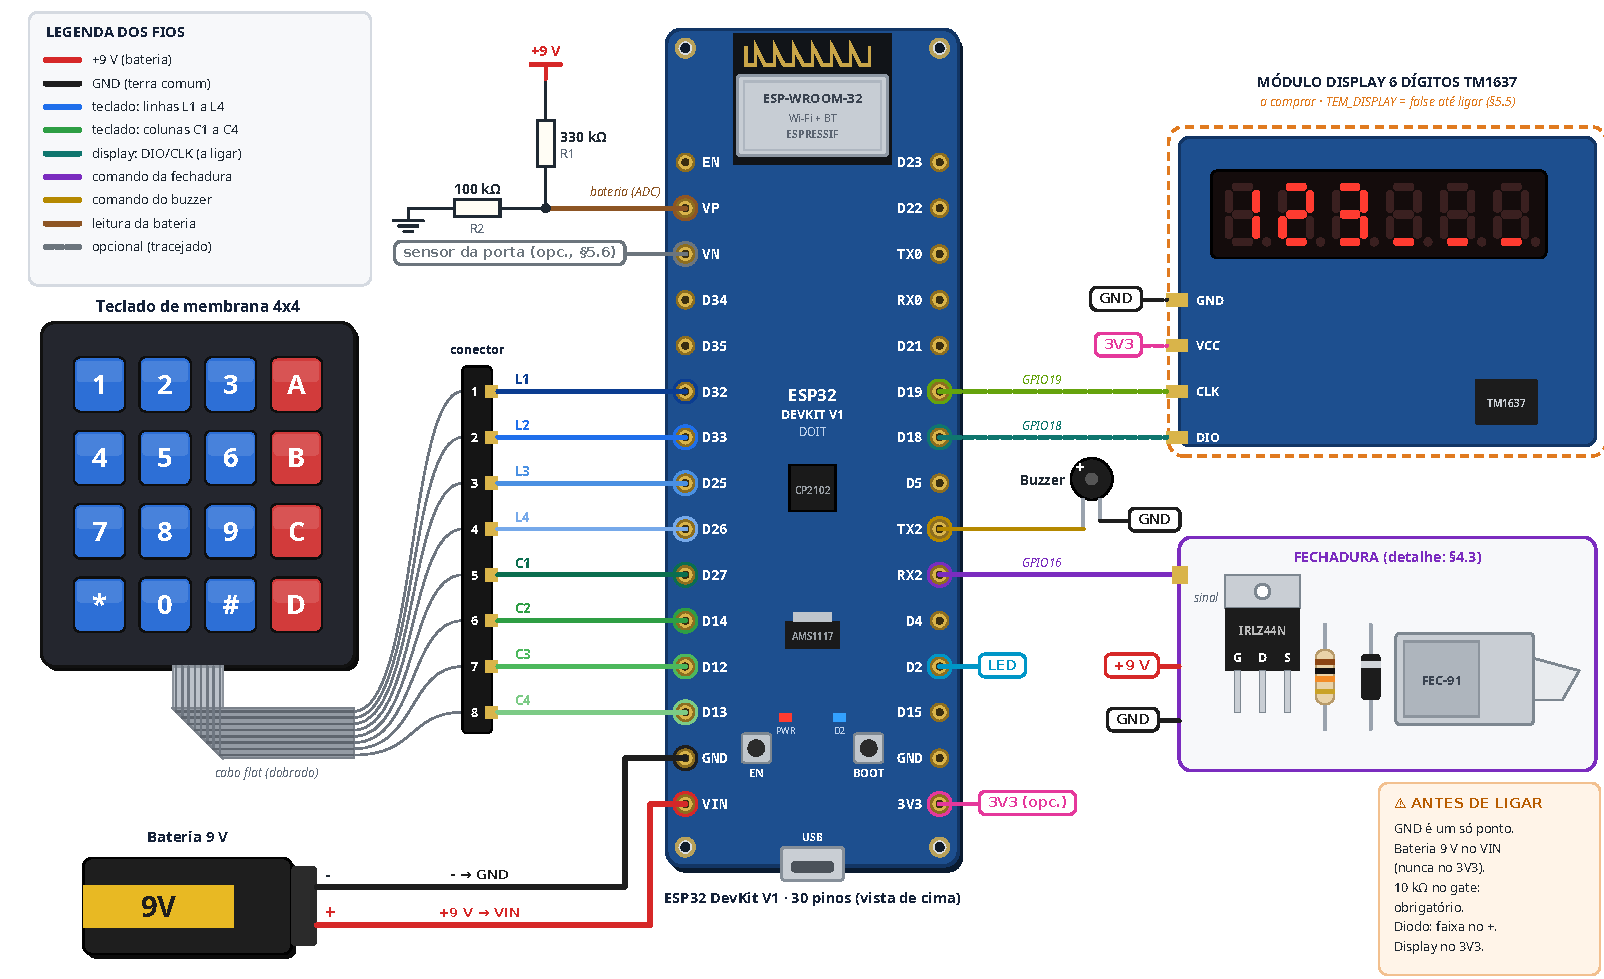
\includegraphics[width=\linewidth]{figuras/diagrama.pdf}
\caption{Diagrama completo de ligação, com a placa desenhada pino a pino.}\label{fig:diagrama}
\end{sidewaysfigure}

\subsection{Alimentação}

A monografia previa uma bateria de lítio de 3,7 V, mas a fechadura FEC-91 que o grupo comprou é de 12 V e não aciona com essa tensão. O grupo testou a fechadura com uma bateria de 9 V e verificou que ela recolhe a lingueta sem problemas. Com isso, a bateria de 9 V alimenta a fechadura diretamente e alimenta o ESP32 pelo pino VIN, cujo regulador interno gera os 3,3 V. Essa escolha eliminou o conversor buck que o grupo chegou a planejar e reduziu a lista de peças.

\subsection{Acionamento da fechadura}

Um pino do ESP32 fornece poucos miliampères e não suporta a corrente da bobina. O grupo usa um MOSFET IRLZ44N como chave no lado do terra, conforme a figura \ref{fig:fechadura}. O pino RX2 controla o gate, um resistor de 10 k$\Omega$ entre o gate e o terra mantém o MOSFET desligado durante o boot e o deep sleep, quando o pino fica em alta impedância, e um diodo 1N4007 em antiparalelo com a bobina absorve o pico de tensão que a bobina gera ao desligar. O IRLZ44N conduz bem com 3,3 V no gate para a corrente dessa fechadura.

\begin{figure}[H]\centering
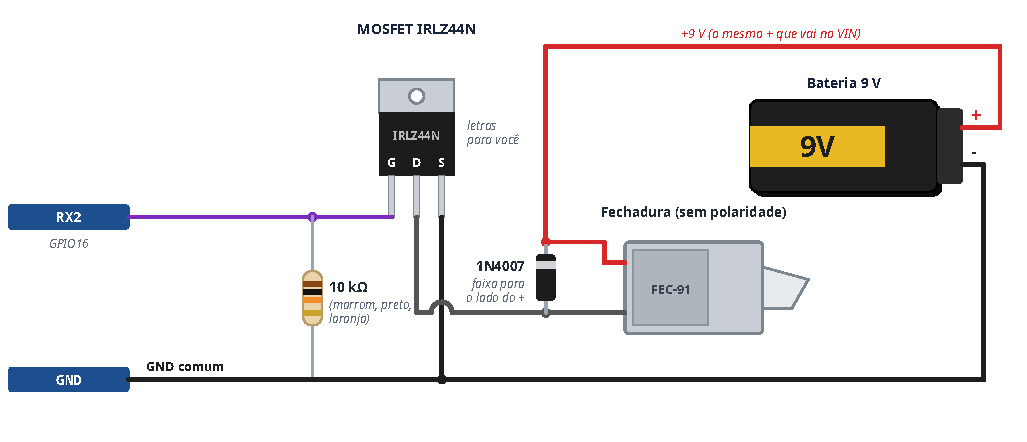
\includegraphics[width=0.9\linewidth]{figuras/fechadura.pdf}
\caption{Montagem do acionamento da fechadura.}\label{fig:fechadura}
\end{figure}

\subsection{Teclado e despertar}

O teclado de membrana 4 por 4 não tem um sinal de tecla pressionada. Cada tecla apenas encosta um fio de linha em um fio de coluna. Com o processador acordado, o firmware energiza uma coluna por vez e lê as linhas. Em deep sleep o processador fica desligado e só o domínio RTC continua ativo, capaz de observar alguns pinos específicos. Para acordar com o teclado, o firmware deixa as quatro colunas em nível alto antes de dormir e configura o despertar por nível alto em qualquer uma das quatro linhas, que usam pinos RTC com pull-down interno. Qualquer tecla então leva uma linha a nível alto e acorda o chip.

Uma das colunas fica no pino D12, que o ESP32 lê no reset para escolher a tensão da memória flash. Nível alto nesse pino seleciona 1,8 V, e a flash da placa, que é de 3,3 V, deixa de funcionar. Para evitar o problema sem mudar a fiação, o grupo gravou o eFuse que fixa a tensão da flash em 3,3 V e faz o chip ignorar o D12 no boot. A seção \ref{sec:problemas} descreve como o grupo validou essa operação antes de executá-la, já que o eFuse é irreversível. O firmware lê o registrador do eFuse no boot e só mantém o D12 em nível alto durante o sono quando o eFuse está gravado, o que protege uma placa nova que ainda não passou pelo procedimento.

\subsection{Buzzer, display e opcionais}

O buzzer ativo de 5 V liga diretamente no pino TX2 e no terra. Com 3,3 V ele apita mais baixo, mas a montagem dispensa transistor e resistores. O display escolhido, um módulo de seis dígitos com o controlador TM1637, faz a multiplexação sozinho e usa apenas dois fios de sinal. O grupo alimenta o módulo pelos 3,3 V da placa, porque os resistores de pull-up do módulo levam as linhas de dados à tensão de alimentação e os pinos do ESP32 não toleram 5 V. Os opcionais incluem o divisor de 330 k$\Omega$ e 100 k$\Omega$ para medir a bateria, um LED externo no D2 e um sensor de porta no VN.

\section{Projeto do software}

\subsection{Organização}

Todo o firmware cabe em um único arquivo, \texttt{src/main.cpp}, com cerca de 550 linhas. O topo do arquivo concentra os parâmetros da monografia, como os tempos, o número de tentativas e os limites do bloqueio, além das constantes de configuração do hardware, como a ordem dos fios do teclado e a presença do display. A tabela \ref{tab:param} lista os principais parâmetros e os valores atuais.

\begin{table}[H]\centering\small
\caption{Parâmetros principais do firmware.}\label{tab:param}
\begin{tabularx}{\linewidth}{@{}l l L@{}}
\toprule
Constante & Valor & Significado \\
\midrule
T\_DEB & 50 ms & Janela de debounce \\
T\_INAT & 15 s & Inatividade que descarta a entrada e leva ao sono \\
T\_ACIO & 5 s & Tempo com a fechadura destravada \\
N\_TENT & 5 & Senhas erradas seguidas até o bloqueio \\
T\_LOCK e T\_MAX & 60 s e 30 min & Bloqueio inicial e teto do bloqueio progressivo \\
W\_REC & 15 min & Janela em que um novo bloqueio conta como consecutivo \\
V\_LOW & 7,0 V & Limiar de bateria fraca \\
TECLADO\_INVERTIDO & verdadeiro & Ordem dos fios do teclado na montagem do grupo \\
TEM\_DISPLAY & falso & Ativa o driver do TM1637 quando o módulo chegar \\
\bottomrule
\end{tabularx}
\end{table}

\subsection{Máquina de estados e laço principal}

O laço principal roda a cada milissegundo. Ele atualiza o padrão de som e luz, lê o teclado, verifica os temporizadores e repassa a tecla lida para o estado atual. Uma função de entrada de estado executa as ações de cada estado uma única vez, como acionar a fechadura no S5 ou sortear o desafio no S1. O firmware reduz o clock da CPU para 80 MHz no boot, porque o teclado e o som não precisam de mais, e chama uma pausa de 1 ms a cada volta do laço para que o sistema operacional coloque o processador em espera.

\subsection{Teclado}

A varredura energiza uma coluna por vez e deixa as demais em alta impedância, para que duas teclas apertadas na mesma linha não coloquem dois pinos em curto. Uma leitura só vale depois de permanecer estável por 50 ms, e o firmware só gera evento na transição de solta para apertada, o que impede repetição ao segurar a tecla. As teclas de limpar e confirmar agem quando o usuário as solta. Esse detalhe permite o combo de 3 s com as duas teclas juntas, que alterna o modo stealth sem disparar a limpeza nem a confirmação. Uma função de mapeamento traduz a posição lida na tecla correta e cobre os dois sentidos possíveis de ligação do cabo do teclado.

\subsection{Persistência}

O firmware guarda uma estrutura de 48 bytes na partição NVS da flash. A estrutura contém um número de sequência, o hash SHA-256 da senha, o estado do modo stealth, o contador de erros, o nível do bloqueio, a indicação de bloqueio em curso, o instante do fim do último bloqueio e um CRC32 dos campos anteriores. Duas chaves guardam duas cópias da estrutura. Cada gravação vai para a cópia inativa, o firmware lê a cópia de volta, confere o conteúdo e só então a promove a ativa. Se a verificação falhar, o firmware repete a gravação até três vezes. No boot, o firmware escolhe a cópia válida com o maior número de sequência e, se nenhuma for válida, assume a senha de fábrica 000000.

O bloqueio sobrevive a resets e à falta de energia. O firmware marca o bloqueio na memória antes de dormir e, ao acordar, retoma o tempo restante. O relógio interno continua contando durante o deep sleep, mas zera quando a energia cai. Nesse caso o firmware recomeça o bloqueio do início, o que pune quem tenta escapar do bloqueio desligando a bateria.

\subsection{Energia}

O cofre entra em deep sleep após 15 s sem tecla e logo depois de trancar. Durante um bloqueio, o firmware dorme com despertar apenas por temporizador, de modo que o teclado não acorda o cofre até o fim do tempo. Fora do bloqueio, o despertar acontece pelo teclado, conforme a seção anterior.

\subsection{Uso de memória}

O grupo compila o firmware com otimização O3, como a especificação do trabalho pede. A tabela \ref{tab:mem} mostra o uso de memória da versão atual, que fica muito abaixo da capacidade da placa e dispensa recorrer à otimização O2.

\begin{table}[H]\centering\small
\caption{Uso de memória com otimização O3.}\label{tab:mem}
\begin{tabular}{@{}l r r r@{}}
\toprule
Memória & Usado (bytes) & Disponível (bytes) & Uso \\
\midrule
Flash (programa) & 315\,625 & 1\,310\,720 & 24,1\,\% \\
RAM & 23\,264 & 327\,680 & 7,1\,\% \\
\bottomrule
\end{tabular}
\end{table}

\section{Protocolos de comunicação}

O cofre não usa rede. O firmware mantém o Wi-Fi e o Bluetooth desligados, o que economiza energia e elimina uma superfície de ataque. Três canais de comunicação aparecem no projeto.

O primeiro é a porta serial UART a 115200 bits por segundo, com 8 bits de dados, sem paridade e 1 bit de parada. O conversor CP2102 da placa transporta essa porta pelo USB. O firmware usa a serial para registrar cada mudança de estado, o que serviu de base para todos os testes, e nunca envia a senha por ela. A mesma porta grava o firmware por meio do protocolo do bootloader em ROM do ESP32, que a ferramenta esptool implementa.

O segundo é o protocolo de dois fios do TM1637. Ele lembra o I2C, mas não tem endereço e transmite cada byte com o bit menos significativo primeiro. O firmware implementa o protocolo por software. Uma condição de início leva o DIO a nível baixo com o CLK em nível alto, cada bit muda com o CLK em nível baixo e o módulo responde com um bit de confirmação ao fim de cada byte. Para enviar o conteúdo, o firmware manda o comando de escrita com endereço automático, o endereço do primeiro dígito seguido dos seis bytes de segmentos e o comando que liga o display com o brilho escolhido. O firmware emula a saída em dreno aberto, levando a linha a nível baixo ativamente e soltando a linha para o nível alto, e só envia dados quando o conteúdo muda.

O terceiro aparece apenas no ambiente de desenvolvimento. Como o grupo trabalha no WSL2 dentro do Windows, a ferramenta usbipd-win encaminha o dispositivo USB da placa para o Linux pelo protocolo USB/IP.

\section{Ferramentas, linguagens e sistema operacional}

O grupo escreveu o firmware em C++ sobre o framework Arduino para ESP32, versão 2.0.17, que por sua vez roda sobre o ESP-IDF 4.4.7 da Espressif. O ESP-IDF já inclui o FreeRTOS, e o laço principal do firmware roda em uma tarefa do FreeRTOS que o framework cria. O firmware não cria tarefas próprias. Uma única tarefa com um laço não bloqueante atende todos os requisitos de tempo do cofre, e o FreeRTOS cuida do escalonamento do sistema e da espera do processador. O compilador é o GCC 8.4.0 para a arquitetura Xtensa.

O PlatformIO Core 6.2 gerencia a compilação, a gravação e o monitor serial, e baixa sozinho o compilador e as bibliotecas na primeira compilação. O grupo usou o esptool para gravar a placa e o espefuse para ler e gravar os eFuses. O desenvolvimento aconteceu no Visual Studio Code, no Ubuntu dentro do WSL2, com o usbipd-win para acessar a placa e o Git com o GitHub para versionar o código. O grupo gerou o guia de montagem e o guia de testes com scripts em Python que usam a biblioteca ReportLab, e escreveu este relatório em \LaTeX. O grupo também usou um assistente de programação baseado em inteligência artificial, o Claude Code, para escrever o firmware, os guias e os testes de diagnóstico, sempre conferindo o resultado na placa.

\section{Interface com o usuário}

O usuário interage com o cofre pelo teclado e recebe retorno por som, luz e, quando o módulo chegar, pelo display. Os dígitos de 0 a 9 servem ao desafio e à senha, a tecla asterisco limpa o que o usuário digitou, a tecla sustenido confirma, a tecla A inicia a troca de senha durante a abertura e o par asterisco e sustenido, segurado por 3 s, alterna o modo stealth. A figura \ref{fig:fluxo} resume o uso normal.

\begin{figure}[H]\centering
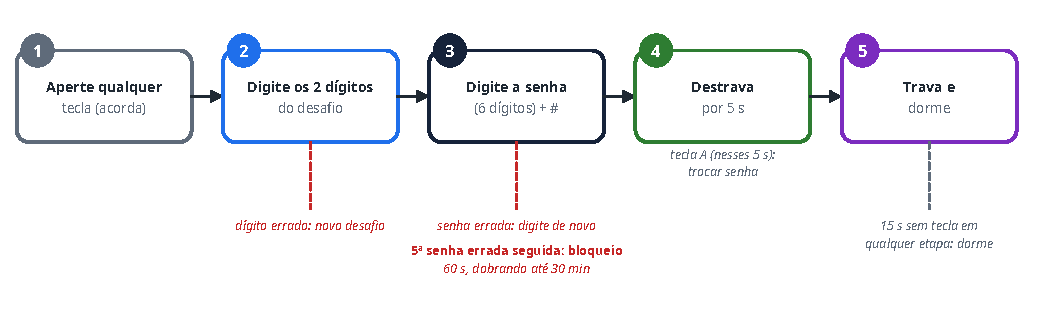
\includegraphics[width=0.95\linewidth]{figuras/fluxo.pdf}
\caption{Uso normal do cofre.}\label{fig:fluxo}
\end{figure}

Como o display ainda não chegou, o cofre mostra o desafio por piscadas do LED acompanhadas de bipes. Cada dígito vira um grupo de piscadas curtas, e o zero vira uma piscada longa, conforme a figura \ref{fig:piscadas}. Quando o display estiver ligado, o desafio aparece no centro do display, e as telas da figura \ref{fig:telas} indicam a senha em digitação, a abertura, o bloqueio e a bateria fraca.

\begin{figure}[H]\centering
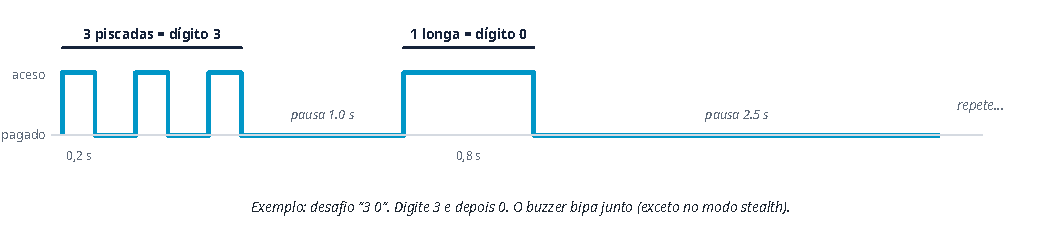
\includegraphics[width=0.95\linewidth]{figuras/piscadas.pdf}
\caption{Desafio em piscadas, sem display.}\label{fig:piscadas}
\end{figure}

\begin{figure}[H]\centering
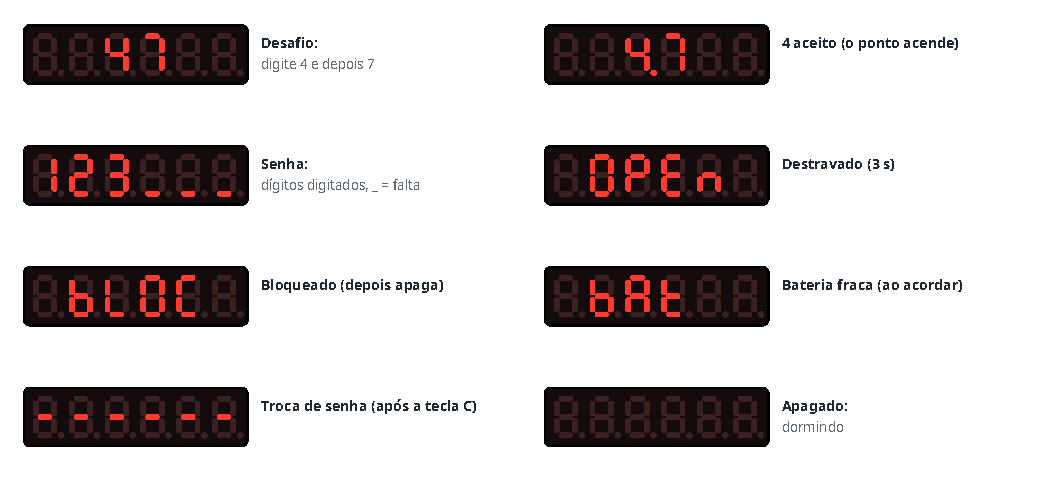
\includegraphics[width=0.9\linewidth]{figuras/telas.pdf}
\caption{Telas previstas para o display de seis dígitos.}\label{fig:telas}
\end{figure}

O buzzer ativo tem um único tom, então o firmware diferencia os eventos pelo número e pela duração dos bipes. Uma tecla aceita gera um bipe curto, um erro gera dois bipes curtos, o acesso gera três bipes de duração crescente, o bloqueio gera um bipe longo e a bateria fraca gera cinco bipes rápidos. No modo stealth o buzzer fica mudo e o LED continua piscando.

\section{Protótipo}

O protótipo atual roda na bancada com a placa ESP32 DevKit V1 ligada ao computador pelo USB, o teclado conectado aos pinos D32 a D13 e um LED com resistor no lugar da fechadura, no pino RX2. Esse arranjo permitiu testar todo o fluxo sem a bateria. Nessa montagem o grupo verificou o desafio, a senha correta acendendo o LED por 5 s, a senha errada, o bloqueio, o sono e o despertar. A fechadura real funciona com a bateria de 9 V, e o grupo testou o acionamento dela diretamente na bateria. A montagem com o MOSFET, a instalação no case e o display seguem pendentes.

\foto{fotos/prototipo_bancada.jpg}{Protótipo em bancada com a placa, o teclado e o LED no lugar da fechadura.}{fig:foto1}
\foto{fotos/fechadura_9v.jpg}{Teste da fechadura com a bateria de 9 V.}{fig:foto2}

Os vídeos do protótipo acompanham este relatório como arquivos MP4 separados na entrega da tarefa. Eles mostram o fluxo completo de abertura com o LED no lugar da fechadura e o acionamento da fechadura pela bateria.

\section{Problemas enfrentados}\label{sec:problemas}

O primeiro problema surgiu na compra dos componentes. A fechadura disponível era de 12 V, enquanto a especificação previa uma bateria de 3,7 V que não aciona essa fechadura. O grupo chegou a projetar a alimentação com uma bateria de 12 V e um conversor buck, mas depois testou a fechadura com uma bateria de 9 V e adotou essa solução, que dispensa o conversor e simplifica a montagem.

O segundo problema envolveu o display. O grupo tinha seis displays de sete segmentos avulsos, de anodo comum, e a placa não tinha pinos livres suficientes para eles. Mesmo multiplexados, seis displays exigiriam catorze pinos. O grupo avaliou uma solução com dois registradores de deslocamento, um driver ULN2803 e seis transistores, mas preferiu comprar um módulo pronto com o controlador TM1637, que usa dois fios. O firmware já tem o driver do módulo, desligado até o módulo chegar, e mostra o desafio por piscadas do LED enquanto isso.

O terceiro problema apareceu no primeiro teste com o teclado. O cofre recusava o desafio logo na primeira tecla. O grupo ligou um modo de diagnóstico que imprime cada tecla lida, apertou as dezesseis teclas em ordem e comparou o resultado. A leitura saiu espelhada, o que mostrou que a ordem dos oito fios estava invertida em relação à numeração que o projeto assumia. Em vez de refazer a fiação, o grupo acrescentou ao firmware uma opção que trata os dois sentidos de ligação.

O quarto problema veio da sequência de pinos do teclado. O grupo queria os oito fios em pinos vizinhos e sem resistores, e a única sequência que atendia ao despertar pelo teclado incluía o pino D12. Como o D12 escolhe a tensão da flash no reset, o firmware precisava manter esse pino em nível baixo durante o sono, e quatro teclas deixavam de acordar o cofre. Para resolver, o grupo gravou o eFuse que fixa a tensão da flash em 3,3 V. Antes de gravar, o grupo conferiu a operação na documentação do esptool, nos datasheets do ESP32 e do módulo WROOM-32 e no guia da ESP-IDF, leu o estado atual dos eFuses da placa, confirmou que a flash da placa já operava em 3,3 V e simulou o comando em um chip virtual para ver exatamente quais bits mudariam. Depois de gravar, o grupo comparou o resultado com a simulação e testou cinco ciclos seguidos de sono e despertar com o D12 em nível alto, todos sem falha.

O quinto problema foi o mais trabalhoso. Durante um teste, o firmware acusou uma falha na verificação de uma gravação na memória. O grupo escreveu testes que gravam dados aleatórios diretamente na flash e conferem a leitura, e as primeiras rodadas mostraram taxas de erro crescentes, chegando a corromper a maior parte das gravações. Uma varredura setor por setor mostrou que o erro dependia do tempo de uso contínuo e não da região da memória. Depois de trocar a porta USB e repetir o teste nas condições reais do cofre, com a CPU a 80 MHz e pausas entre as gravações, nenhuma gravação falhou. O grupo concluiu que a porta USB antiga fornecia energia instável sob carga contínua e acrescentou ao firmware a repetição automática da gravação, como proteção extra.

Por fim, o ambiente de desenvolvimento também exigiu ajustes. O WSL2 não enxerga dispositivos USB sem o usbipd-win, o kernel do WSL não carregava o driver do conversor CP2102 automaticamente e a porta serial aparecia sem permissão de acesso a cada reconexão. O grupo documentou os comandos de cada etapa no guia de montagem. Uma atualização recente de uma biblioteca Python também quebrou a ferramenta de eFuses, e o grupo fixou a versão anterior da biblioteca.

\section{Cronograma}

A tabela \ref{tab:crono} compara o cronograma previsto com o realizado até a data deste relatório. As datas realizadas vêm do histórico do repositório e dos registros de teste do grupo.

\begin{table}[H]\centering\small
\caption{Cronograma previsto e realizado.}\label{tab:crono}
\begin{tabularx}{\linewidth}{@{}L l l@{}}
\toprule
Etapa & Previsto & Realizado \\
\midrule
Especificação de requisitos e monografia & (preencher) & setembro de 2026 \\
Escolha e compra dos componentes principais & (preencher) & setembro de 2026 \\
Primeira versão do firmware e repositório & (preencher) & 25/09/2026 \\
Guia de montagem e primeiros testes na placa & (preencher) & 09/10/2026 \\
Diagnóstico do teclado e da memória flash & (preencher) & 09/10 a 11/10/2026 \\
Ajustes da máquina de estados e gravação do eFuse & (preencher) & 11/10/2026 \\
Alimentação por bateria de 9 V e guia de testes & (preencher) & 11/10/2026 \\
Melhorias no firmware & (preencher) & 13/10/2026 \\
Relatório técnico de progresso & (preencher) & 15/10/2026 \\
Chegada e teste do display TM1637 & (preencher) & pendente \\
Montagem no case e testes de aceitação completos & (preencher) & pendente \\
\bottomrule
\end{tabularx}
\end{table}

\section{Próximos passos}

O grupo ainda precisa montar o acionamento da fechadura com o MOSFET, instalar o conjunto no case de MDF com a bateria acessível por fora, ligar e testar o display assim que ele chegar e executar os 33 casos do guia de testes na montagem final. Também falta decidir se o grupo instala o sensor de porta e o divisor de bateria, que o firmware já suporta. A questão da autonomia fica registrada como limitação da placa de desenvolvimento.

\begin{thebibliography}{9}
\bibitem{mono} GRUPO 7. Projeto Talos: cofre eletrônico com ESP32. Monografia, PCS3848 Sistemas Embarcados, Escola Politécnica da USP, 2026.
\bibitem{ds} ESPRESSIF SYSTEMS. ESP32 Series Datasheet, versão 5.3. Disponível em: \url{https://documentation.espressif.com/esp32_datasheet_en.pdf}.
\bibitem{wroom} ESPRESSIF SYSTEMS. ESP32-WROOM-32 Datasheet. Disponível em: \url{https://documentation.espressif.com/esp32-wroom-32_datasheet_en.pdf}.
\bibitem{idf} ESPRESSIF SYSTEMS. ESP-IDF Programming Guide, versão 4.4.7. Disponível em: \url{https://docs.espressif.com/projects/esp-idf/en/v4.4.7/esp32/}.
\bibitem{esptool} ESPRESSIF SYSTEMS. esptool e espefuse: Set Flash Voltage. Disponível em: \url{https://docs.espressif.com/projects/esptool/en/release-v4/esp32/espefuse/set-flash-voltage-cmd.html}.
\bibitem{ganssle} GANSSLE, J. A Guide to Debouncing. 2008. Disponível em: \url{https://www.ganssle.com/debouncing.htm}.
\end{thebibliography}

\end{document}
